\subsection{Remote Vision Virtual Subsystem}%
\label{sec:remote-visi-subsyst-testing}
In this section are presented the tests performed on the \gls{rvvs} subsystem in
the relevant domains.
%
\subsubsection{Image Acquisition}%
\label{sec:img-acq-rvvs-test}
The image acquisition system, implemented in
Section~\ref{sec:img-acq-rvvs-implem}, was tested out to assess its behaviour.

Firstly, it was selected the built-in webcam from host and attached to the guest
\gls{vm}. However,
and despite extensive troubleshooting, the bypass suggested for web
cameras\cite{webcam-bypass} was not possible for a Mac OS host. Thus, a quick
alternative was to flash a Linux \gls{os} onto a \gls{sd} card and plug it to a
Raspberry Pi 3 (available) and connect an external \gls{usb} camera to it (Fig.~\ref{fig:rasp-cam-test}).
% Raspberry Pi 3 camera test
\begin{figure}[!hbt]
\centering
    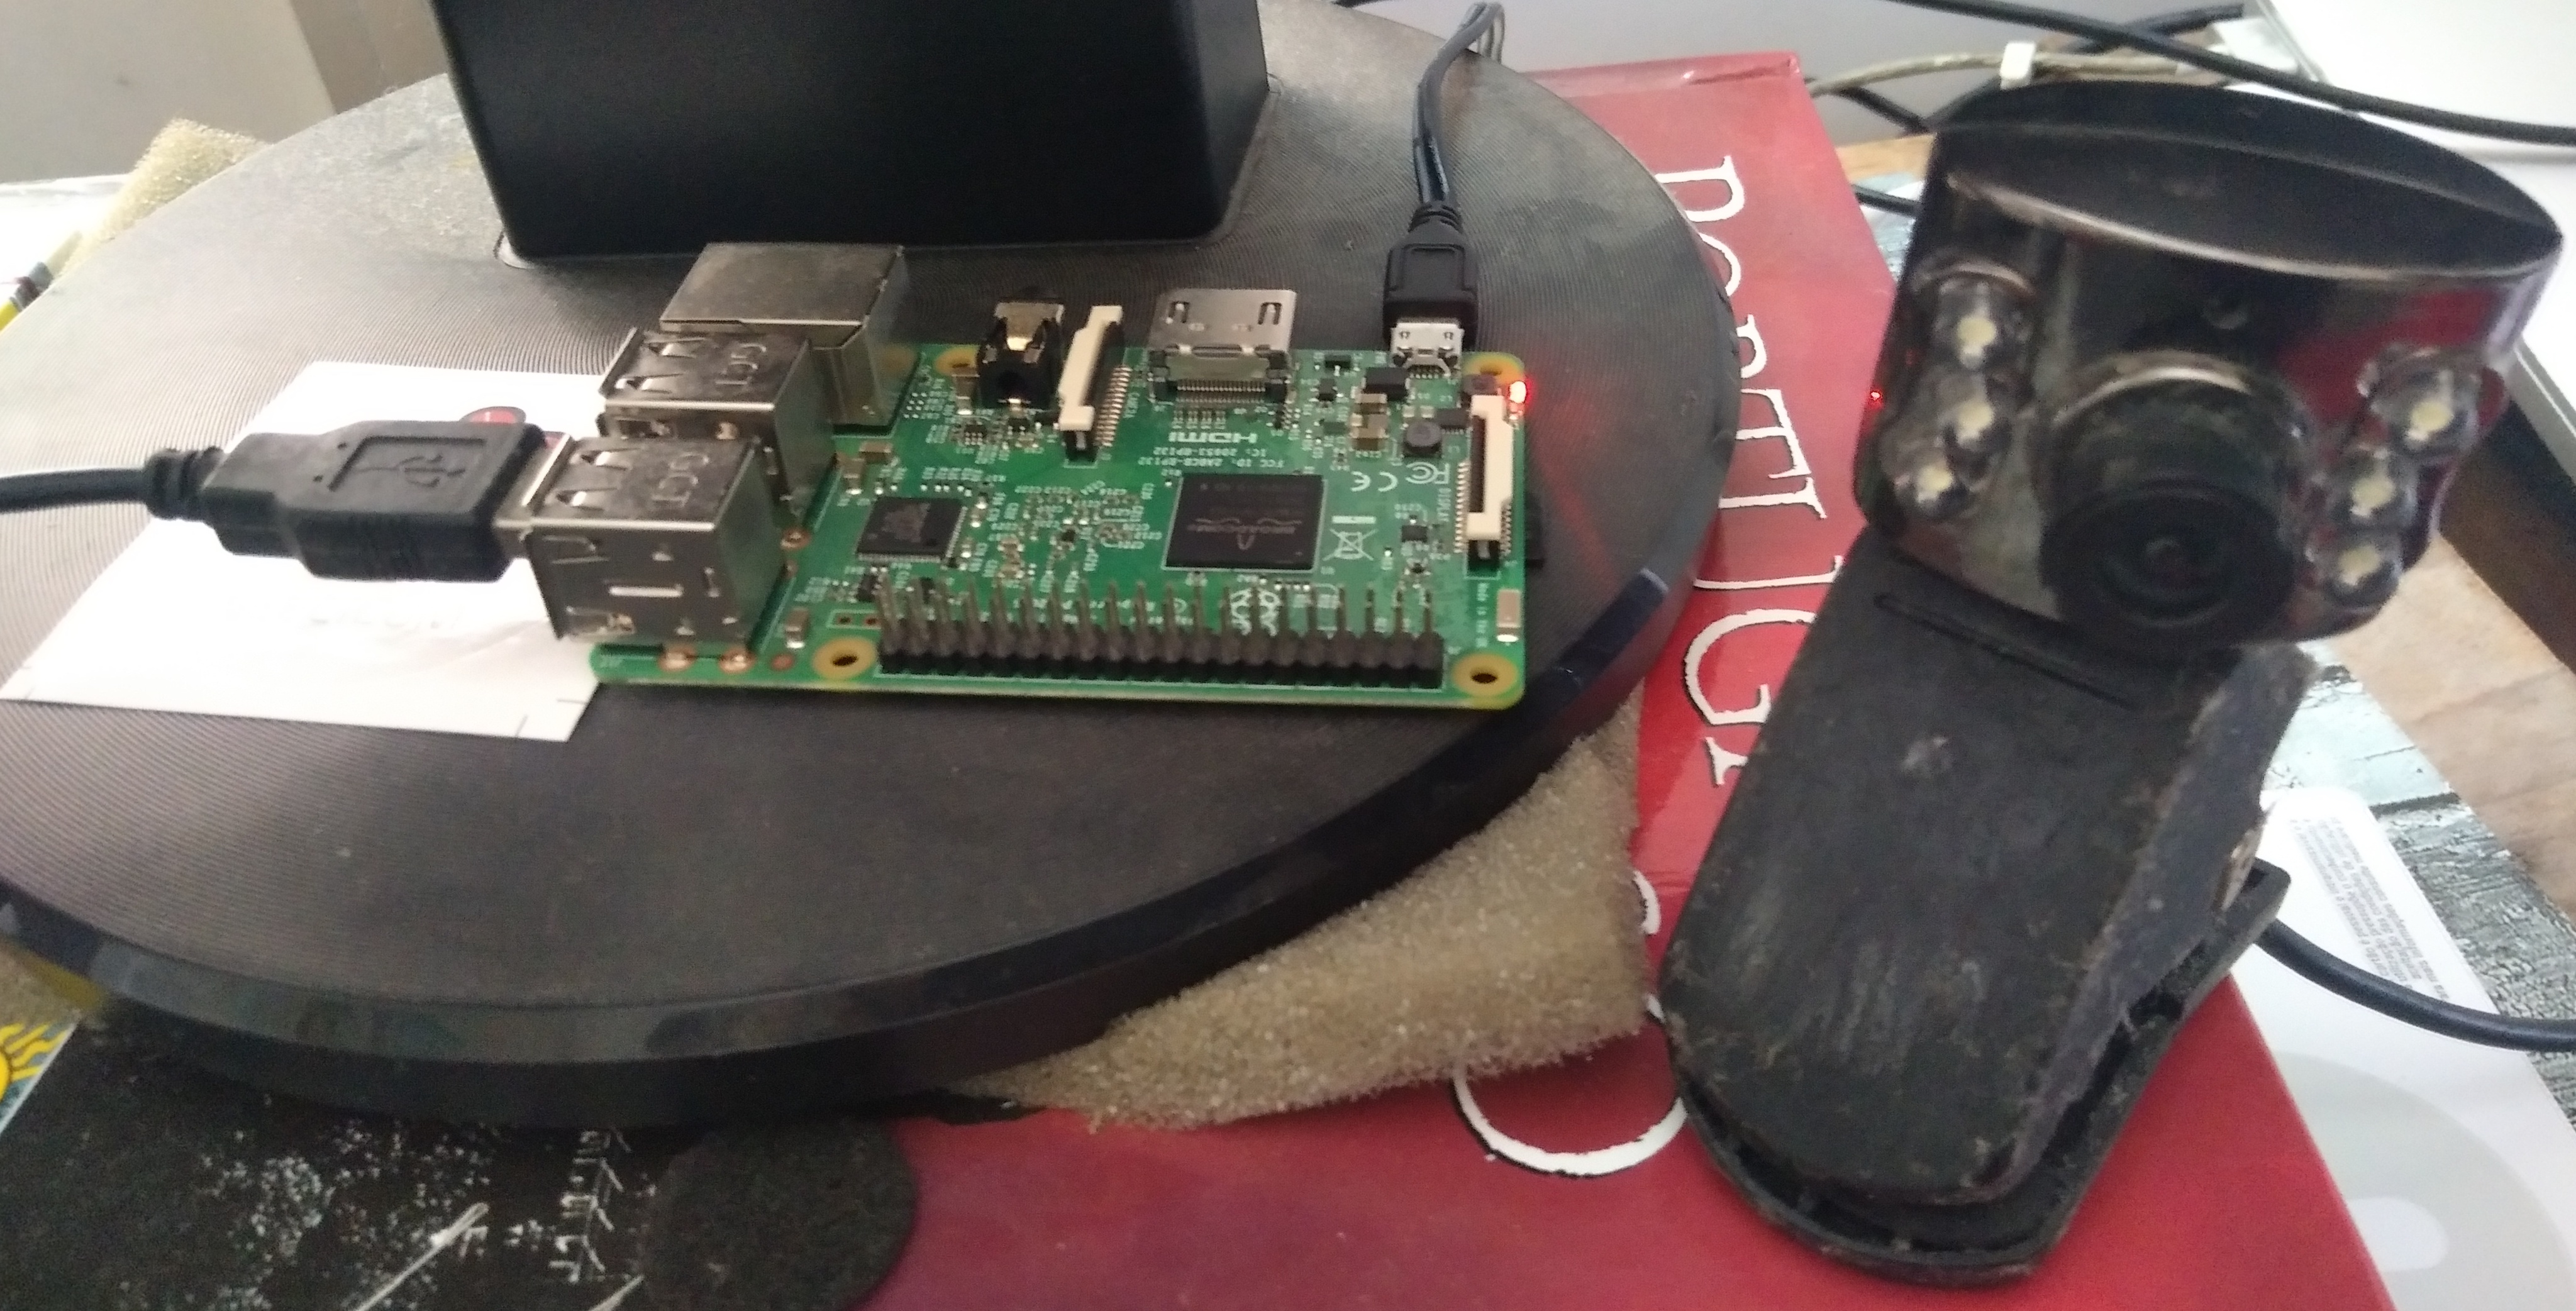
\includegraphics[width=0.6\textwidth]{./img/rasp-cam-test.jpg}
  \caption{Raspberry Pi 3 + Webcam testing setup}%
\label{fig:rasp-cam-test}
\end{figure}
%

The deployment was performed using the \gls{ssh} protocol to connect to the
Raspberry Pi and execute the necessary commands on it, and using the \gls{scp}
command that uses the \gls{sftp} protocol to transfer files between host and
guest (Listing~\ref{lst:deploy-cmds}).
\lstinputlisting[language=sh, caption={Deployment commands targetting Raspberry
Pi},label=lst:deploy-cmds,
style=customc]{./listing/ssh-scp.sh}%

The web camera was then tested using the \texttt{lsusb} command and piping the
output to a \texttt{.txt} file for further
examination. Listing~\ref{ref:lst:lsb-output} contains an excerpt of this output
where it can be observed the
webcam model (\texttt{Cubeternet WebCam}) and the \gls{usb}2.0 interface.
\lstinputlisting[language=sh, caption={Webcam information obtained via
  \texttt{lsusb} (excerpt)},label=lst:lsb-output,
style=customc]{./listing/lsusb-output.sh}%

However, this information by itself is not so useful. Additionally, and much
more importantly, one wants to check the capabilities of the device and the
supported formats. For that purpose it was used the \texttt{v4l2-ctl} utility
(Listing~\ref{lst:webcam-features}). It can be observed that the only format
supported is YUYV, which is a colour space based on one luminance component (Y')
and two chrominance components, called U(blue) projection and V(red projection),
respectively. The framerate is also fixed (30 fps), but with different
resolutions. This is very limitative, as the newer webcams support MJPEG
formats, easing video capture.
\lstinputlisting[language=sh, caption={Webcam supported image formats,
  resolutions, and framerates},label=lst:webcam-features,
style=customc]{./listing/webcam-features.sh}%

Effectively, it was executed the driver program for the webcam interface
(Listing~\ref{lst:webcam-main}), but it reported the unsupported format as
expected (Listing~\ref{lst:webcam-main-error}).
% webcam-main-error
\lstinputlisting[language=C++, caption={Webcam driver program error: unsupported
image format},label=lst:webcam-main-error,
style=customc]{./listing/webcam-main-error.sh}%

Then, it was tried out the \texttt{UYVY422} format by modifying the following
lines into Listing~\ref{lst:webcam-main}
(Listing~\ref{lst:webcam-main-modifs})
% webcam-main-error
\lstinputlisting[language=C++, caption={Webcam driver program error:
  modifications to support \texttt{UYVY422} format},label=lst:webcam-main-modifs,
style=customc]{./listing/webcam-main-modifs.cpp}%

Although an image in the \texttt{UYVY422} format was obtained, \texttt{ffmpeg}
requires tedious conversions between the packed format (\texttt{UYVY422}) to
planar one (\texttt{JPG}). Thus, an online tool was used to convert this image~\cite{conv-UYVY-jpg} into \texttt{jpg} format. In Fig.~\ref{fig:rasp-cam-test-succ} can be seen that an image was
successfully acquired.
% Raspberry Pi 3 camera test
\begin{figure}[!hbt]
\centering
    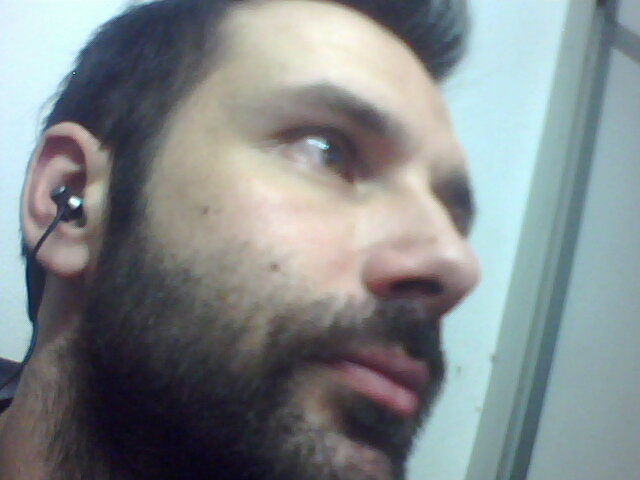
\includegraphics[width=0.6\textwidth]{./img/webcam-test-success.jpg}
  \caption{Raspberry Pi 3 + Webcam test: success}%
\label{fig:rasp-cam-test-succ}
\end{figure}

However, this is a tedious process that could be avoided by using a different,
newer, web camera supporting additional formats and resolutions, which limited
severely the implementation and testing.
%
%%% Local Variables:
%%% mode: latex
%%% TeX-master: "../../../dissertation"
%%% End:
